

\chapter{Brechungsindex von Glas}
\label{v:9}

In diesem Versuch betrachten Sie die Brechung und Reflexion von Licht im Medium am Beispiel eines Glasprismas.

%------------------------------------------------
\section{Stichworte}
%------------------------------------------------

Reflexion; Brechungsgesetz; Totalreflexion; Dispersion; Brechungsindex; Minimalablenkwinkel.
%
%------------------------------------------------
\section{Literatur}
%------------------------------------------------

Gehrtsen, Kapitel 9.1.2 - 9.1.5
%
%------------------------------------------------
\section{Anwendungsbeispiele}
%------------------------------------------------

Linsen, Lichtleiter, Auge, Spektroskopie, Regenbogen.

%------------------------------------------------
\section{Theoretischer Hintergrund}
%------------------------------------------------

F�llt Licht auf die Grenzfl�che zwischen zwei Medien (z.B. Luft und Glas), so kann es entweder reflektiert werden oder es dringt unter �nderung von Richtung, Geschwindigkeit und Wellenl�nge ein. Ein Ma� f�r diese �nderung ist der Brechungsindex $n$. Die Tatsache, dass $n$ f�r verschiedenfarbiges Licht verschieden ist, bezeichnet man als Dispersion; d.h. violettes Licht (kurze Wellenl�nge) wird st�rker abgelenkt als rotes Licht. % Den Studenten ist meistens nicht klar, dass Reflexion und Brechung gleichzeitig stattfinden k�nnen. In diesem Zusammenhang kann man auch den Winkel der Totalreflexion erw�hnen. Man sollte auch unbedingt den gebrochenen Strahl benennen. Mein Vorschlag: F�llt Licht auf die Grenzfl�che zwischen zwei Medien (z.B. Luft und Glas), wird ein Teil des Lichts reflektiert und der Rest dringt unter �nderung von Richtung, Geschwindigkeit und Wellenl�nge in das andere Medium ein (gebrochener Strahl). Ein Ma� f�r diese �nderung ist der Brechungsindex $n$. Die Tatsache, dass $n$ f�r verschiedenfarbiges Licht verschieden ist, bezeichnet man als Dispersion; d.h. violettes Licht (kurze Wellenl�nge) wird st�rker abgelenkt als rotes Licht. Ist der Einfallswinkel gr��er als der Grenzwinkel der Totalreflexion, wird das gesamte Licht reflektiert.
 

\subsection{Das Huygens-Fresnel'sche Prinzip}

Die Wellenausbreitung im homogenen Medium und auch in komplizierteren F"allen l"a{\ss}t sich relativ intuitiv verstehen, wenn man sich nach \textit{Huygens} vorstellt, dass in jedem Punkt einer Wellenfront ein Streuzentrum sitzt, von welchem Kugelwellen (\textit{Elementarwellen}) ausgehen. Diese "uberlagern sich dann zu einer neuen Wellenfront.\\
F"allt eine ebene Welle schr"ag auf die ebene Grenze zwischen zwei Medien, in denen die Wellen unterschiedliche Ausbreitungsgeschwindigkeiten $c_1$ und $c_2$ haben, so haben die Elementarwellen in den beiden Medien nach einer bestimmten Zeit unterschiedliche Radien, welche sich wie $c_1/c_2$ verhalten. Damit nehmen die "Uberlagerungen der Elementarwellen, welche in dem jeweiligen Medium wieder ebene Wellenfronten bilden, verschiedene Winkel zum Lot auf die Grenzfl"ache ein. Damit erhalten wir das allgemeing"ultige Brechungsgesetz
\begin{equation} \label{eq:Brechungsgesetz}
\frac{\sin\alpha}{\sin\beta} = \frac{c_1}{c_2}
\end{equation}

\subsection{Brechungsindex und Snellius'sches Brechungsgesetz}

Der Brechungsindex $n$ eines Mediums kann "uber die Geschwindigkeit der Lichtwellen in diesem Medium definiert werden als:
\begin{equation}
n = \frac{c_0}{c_m}\, ,
\end{equation}
wobei $c_0$ die Lichtgeschwindigkeit im Vakuum bezeichnet und $c_m$ die Lichtgeschwindigkeit im Medium.\\

\noindent
Mit dieser Definition wird aus Gleichung \ref{eq:Brechungsgesetz} das \textit{Snellius'sche Brechungsgesetz}
\begin{equation} \label{eq:Snellius}
\frac{\sin\alpha_1}{\sin\alpha_2} = \frac{n_2}{n_1} = \frac{c_1}{c_2} = \frac{\lambda_1}{\lambda_2}
\end{equation}

\subsection{Ein paar Worte zum Prisma}

Wenn ein Lichtstrahl symmetrisch durch das Prisma hindurchgeht, d.h. parallel zur Grundkante, erf�hrt er die kleinste Ablenkung (Minimal-Ablenkungswinkel). In diesem Fall l�sst sich eine geometrische Beziehung zwischen dem Brechungsindex $n$ des Prismas, dem brechenden Winkel $\gamma$ des Prismas und dem Minimalablenkungswinkel $\delta$ aufstellen:
\begin{equation}
n = \frac{\sin\left(\frac{\delta + \gamma}{2}\right)}{\sin\left(\frac{\gamma}{2}\right)}
\end{equation}
%------------------------------------------------
\section{Fragen zur Vorbereitung}
%------------------------------------------------

\begin{enumerate}
 %
 \item Was soll heute im Praktikum gemessen werden? Warum?
 %
 \item Welchen physikalischen Vorgang beschreibt das Snellius'sche Brechungsgesetz?
 %
 \item Wie ist der Brechungsindex definiert? (Tip: Lichtgeschwindigkeit)
 %
 \item Wie h"angen Wellenl"ange und Frequenz einer Lichtwelle zusammen?
 %
 \item Was ist Dispersion?
 %
 \item Wann kann man Totalrefelxion beobachten?
 %
 \item Wie l"asst sich der Winkel f"ur die Totalreflexion aus dem Snellius'schen Brechungsgesetz ableiten?
 %
 \item Was f"ur eine Gr"o{\ss}e soll im Versuch bestimmt werden?
 %
 \item Wird im Prisma rotes oder blaues Licht st"arker abgelenkt?
 %
\end{enumerate}

%------------------------------------------------
\section{Durchf�hrung} 
%------------------------------------------------

Im Versuch wird der Brechungsindex n eines Glasprismas bestimmt, das auf einer Apparatur steht, mit der man Winkel zwischen Lichtstrahlen sehr genau messen kann.

\begin{enumerate}
 %
 \item Herstellung von parallelem Licht\\
  Dieser Versuchsteil muss sorgf"altig nach Anleitung durchgef�hrt werden, sonst werden Sie sp"ater keine vern�nftigen Ergebnisse erhalten !
  \begin{itemize}
   \item Nehmen Sie das Okular aus dem Fernrohr und stellen Sie das Fadenkreuz bei entspanntem Auge scharf. Schauen Sie dazu am besten gegen einen strukturlosen Hintergrund.
   \item Setzen Sie das Okular wieder ein und stellen Sie das Fernrohr am offenen Fenster auf unendlich ein. Jetzt sehen Sie gleichzeitig das Fadenkreuz und weit entfernte Gegenst"ande scharf und parallaxenfrei (bei seitlicher Bewegung des Auges verschiebt sich das Fadenkreuz nicht gegen den Hintergrund). \\
   Mit dieser Einstellung wird paralleles Licht im Auge fokussiert.
   \item Stellen Sie nun das Fernrohr direkt in den Strahlengang und verschieben Sie den Spalt so lange, bis Sie ihn durch das Fernrohr scharf sehen. Damit haben Sie den Spalt so eingestellt, dass er paralleles Licht emittiert.
  \end{itemize}
  Das Fernrohr kann geschwenkt und die Stellung auf einer Gradeinteilung abgelesen werden. Die Einteilung der Scheibe ist auf 0,50 genau. Der Nonius umfasst 60 Skalenteile, so dass man auf 0,50 genau ablesen kann.\\
  Der Spalt sollte aus Intensit�tsgr�nden nicht zu eng eingestellt werden. Der Spalt sollte breiter sein als der Doppelstrich im Fernrohr.
 %
 \item Messen Sie den (doppelten) brechenden Winkel $2\,\gamma$ des Prismas mit reflektiertem Licht. Wiederholen Sie die Messung drei Mal.
 %
 \item Messen Sie den (doppelten) minimalen Ablenkwinkel $2\,\delta$ f"ur die gelbe He-Linie ($\lambda = 587,5$\,nm) und die blaue He-Linie ($\lambda = 447,2$\,nm). Wiederholen Sie die Messungen jeweils drei Mal. \\
 Den minimalen Ablenkwinkel erkennt man wie folgt: Beobachtung der gelben He-Linie. Das Prisma wird in eine Richtung gedreht. Dabei erkennt man, dass diese Linie �ber eine bestimmte Stelle nicht hinauswandert. Diese Stelle ist diejenige, die dem Winkel der Minimalablenkung zugeordnet werden kann. % Hier haben die allermeisten Studenten gro�e Probleme bei der Durchf�hrung, deswegen mehr Info. Vorschlag: Den minimalen Ablenkwinkel erkennt man wie folgt: Beobachtung der gelben He-Linie. Drehen sie das Prisma so lange in eine Richtung, dass der Ablenkwinkel minimiert wird, d.h. der Winkel zwischen einfallendem Strahl und austretendem Strahl wird minimal. Dies entspricht einem der zwei Strahleng�nge in Bild x.x. Haben sie diesen Strahlengang hergestellt, liegt die beobachtete gelbe Linie auf einem Umkehrpunkt, d.h. die Linie wandert nicht �ber diesen Punkt hinaus, wenn sie das Prisma nun hin und her drehen. Messen sie anschlie�end den minimalen Ablenkwinkel f�r den zweiten gezeigten Strahlengang. Wiederholen sie nun die Messung f�r 2$\delta$ drei Mal.  
 \item Beobachten Sie das Spektrum der Wasserstoff-Lampe.
\end{enumerate}
\begin{figure}[ht]
	\centering
		%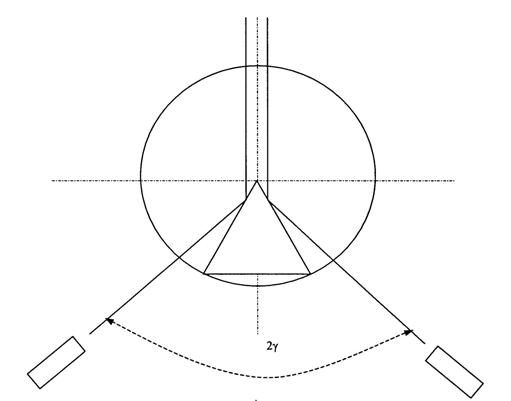
\includegraphics[width=.45\textwidth]{Versuch_9-10/Abbildungen/prisma1.JPG}
		%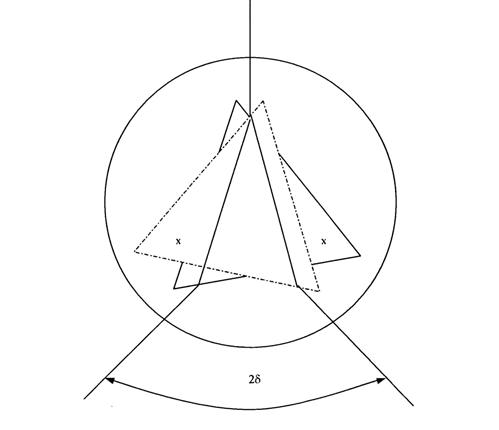
\includegraphics[width=.42\textwidth]{Versuch_9-10/Abbildungen/prisma2.JPG}
	\caption{Links: Strahlengang des reflektierten Lichts, einmal rechts, einmal links von der brechenden Kante. Rechts: Bestimmung des minimalen Ablenkwinkels.} % Hier mehr Info. Vorschlag: Rechts: Bestimmung des minimalen Ablenkwinkels. Der Ablenkwinkel wird minimal, wenn der gebrochene Strahl parallel zur Grundkante des Prismas verl�uft. Gezeigt ist der \textbf{doppelte}} Ablenkwinkel.
	\label{fig:prisma1}
\end{figure}


%------------------------------------------------
\section{Auswertung} 
%------------------------------------------------

\begin{enumerate}
 %
 \item Berechnen Sie den Mittelwert des brechenden Winkels $\overline{\gamma}$ inklusive seines Fehlers.
 %
 \item Berechnen Sie die Mittelwerte des minimalen Ablenkwinkels $\overline{\delta}$ f"ur die gelbe und die blaue Heliumlinie inklusive der Fehler.
 %
 \item Nehmen Sie an, dass der Brechungsindex von Luft $n=1,0$ betr"agt. Berechnen Sie den Brechungsindex des Glases f"ur die gelbe und die blaue Heliumlinie, inklusive des jeweiligen Fehlers. % Hier ein kleiner Zusatz. Die meisten geben einen Fehler an, der die Einheit Grad hat und schlagen das auf den Brechungsindex drauf. Der Fehler ist dann viel zu gro� und die Studenten diskutieren  die gesamte Messung schlecht. Vorschlag: Beachten sie bei der Fehlerangabe, dass der Brechungsindex keine Einheit hat!
 %
\end{enumerate}


